\documentclass[a4paper,10pt]{article}\usepackage[]{graphicx}\usepackage[]{color}
%% maxwidth is the original width if it is less than linewidth
%% otherwise use linewidth (to make sure the graphics do not exceed the margin)
\makeatletter
\def\maxwidth{ %
  \ifdim\Gin@nat@width>\linewidth
    \linewidth
  \else
    \Gin@nat@width
  \fi
}
\makeatother

\definecolor{fgcolor}{rgb}{0.345, 0.345, 0.345}
\newcommand{\hlnum}[1]{\textcolor[rgb]{0.686,0.059,0.569}{#1}}%
\newcommand{\hlstr}[1]{\textcolor[rgb]{0.192,0.494,0.8}{#1}}%
\newcommand{\hlcom}[1]{\textcolor[rgb]{0.678,0.584,0.686}{\textit{#1}}}%
\newcommand{\hlopt}[1]{\textcolor[rgb]{0,0,0}{#1}}%
\newcommand{\hlstd}[1]{\textcolor[rgb]{0.345,0.345,0.345}{#1}}%
\newcommand{\hlkwa}[1]{\textcolor[rgb]{0.161,0.373,0.58}{\textbf{#1}}}%
\newcommand{\hlkwb}[1]{\textcolor[rgb]{0.69,0.353,0.396}{#1}}%
\newcommand{\hlkwc}[1]{\textcolor[rgb]{0.333,0.667,0.333}{#1}}%
\newcommand{\hlkwd}[1]{\textcolor[rgb]{0.737,0.353,0.396}{\textbf{#1}}}%
\let\hlipl\hlkwb

\usepackage{framed}
\makeatletter
\newenvironment{kframe}{%
 \def\at@end@of@kframe{}%
 \ifinner\ifhmode%
  \def\at@end@of@kframe{\end{minipage}}%
  \begin{minipage}{\columnwidth}%
 \fi\fi%
 \def\FrameCommand##1{\hskip\@totalleftmargin \hskip-\fboxsep
 \colorbox{shadecolor}{##1}\hskip-\fboxsep
     % There is no \\@totalrightmargin, so:
     \hskip-\linewidth \hskip-\@totalleftmargin \hskip\columnwidth}%
 \MakeFramed {\advance\hsize-\width
   \@totalleftmargin\z@ \linewidth\hsize
   \@setminipage}}%
 {\par\unskip\endMakeFramed%
 \at@end@of@kframe}
\makeatother

\definecolor{shadecolor}{rgb}{.97, .97, .97}
\definecolor{messagecolor}{rgb}{0, 0, 0}
\definecolor{warningcolor}{rgb}{1, 0, 1}
\definecolor{errorcolor}{rgb}{1, 0, 0}
\newenvironment{knitrout}{}{} % an empty environment to be redefined in TeX

\usepackage{alltt}
\usepackage{a4wide}
\usepackage{amsmath}
\usepackage{amssymb}
\usepackage[english]{babel}
\usepackage{eurosym}
\usepackage{inputenc}
\usepackage{graphicx}
\usepackage[linesnumbered,ruled]{algorithm2e}
\usepackage{enumerate}
\usepackage{caption}
\usepackage{float}

\title{An analysis on the Metropolis-Hastings algorithm for various iterations}
\author{Kenneth Ruiter (12206909)}
\IfFileExists{upquote.sty}{\usepackage{upquote}}{}
\begin{document}
% setting global settings and loading useful libraries


\maketitle
\newpage

\tableofcontents
\newpage

\section{Introduction}

In statistics, being able to draw from any distribution you like is a very useful tool for analysing your data. Aside from just the 'usual' distributions, some user-defined ones can be hard to sample from directly, when their density is somewhat odd. A well-known way of solving this problem, is by using the Metropolis-Hastings algorithm. This algorithm is a so-called MCMC (Markov Chain Monte Carlo) method to get random samples from such a difficult distribution. In this report we will focus on a particular example of the Metropolis-Hastinds algorithm. We will use the algorithm to estimate the parameters of a simple Ordinary Least Squares regression model, as to easily compare them with the analyitically computed values of the estimates. We will focus on the accuracy of the algorithm by comparing the outputs for a different number of iterations used to compute our estimate.

\subsection{Overview of the report}
In Section~\ref{AD}, we will give more elaborate discription of the Metropolis-Hastings algorithm. We will not explain why it works, however we will go through the algorithm step-by-step. Afterwards, we will randomly generate the data and define some parameters in Section~\ref{Set}. Finally, the results of the algorithm will be shown and discussed in Section~\ref{Res}.

\newpage
\section{Algorithm Description}\label{AD}

In this section, the steps involved in the Metropolis-Hastings algorithm will be discussed, using pseudo-code. For this, let $f(x)$ be the density of the distribution that we want to sample from, also known as the target distribution. We will need an initial draw from our sample, so we arbitrarily take $x_0$. We also need an arbitrary second distribution, that we can easily sample from, with density $g(x)$. This distribution will suggest a new candidate for the following draws. We usually take a symmetric distribution, like the Normal distribution, because it makes it easy to compute the acceptance rate of the candidates. This distribution is ususally called the jumping distribution, or sometimes the proposal distribution. The actual steps of the algorithm are shown now.

\begin{algorithm}[H]
    \SetKwInOut{Input}{Input}
    \SetKwInOut{Output}{Output}

    \underline{function run\_metropolis\_MCMC} $(f, g, x_0, iterations)$\;
    \Input{Density function of target distribution $f$, density function of jumping distribution $g$, initial draw $x_0$, number of iterations $iterations$.}
    
    \Output{A vector of the ordered accepted draws, representing draws from the target distribution.}
    Create a 2-dimensional array, called \emph{chain}, with (\emph{iterations}+1) rows and 3 columns\;
    Set the elements of the first row of \emph{chain} to $x_0$\;
    \For{$i$ in $1:iterations$}
      {
        Create a \emph{proposal} vector, equal to $g(\text{first row of } chain)$\;
        Create a variable, \emph{propab}, which is the probability of accepting the proposal. Set it equal to $\exp{(f(proposal) - f(\text{first row of } chain))}$\;
      \uIf{A Uniformly distributed random variable on the interval $[0,1] < probab$}
        {
          Set the next row of \emph{chain}, $chain[i+1,]$, equal to \emph{proposal}\;
        }
      \uElse
        {
          Set the next row of \emph{chain}, $chain[i+1,]$, equal to the last row, $chain[i,]$\;
        }
      }
    Return $chain$\;
    \caption{The Metropolis-Hastings algorithm}
\end{algorithm}



\newpage
\section{Setup}\label{Set}
In this section we will explain the setup of the experiment. In order to examine the accuracy of the algorithm, we first need a scenario to use the algorithm in. For this, we decide to look at a simple Linear Model example, where the parameters are usually estimated by the Ordinary Least Squares (OLS) method. In this experiment however, we will estimate the parameters using the Metropolis-Hastings algorithm instead, afterwards we are able to compare our findings with the OLS estimators. To create this scenario, we first need a linear model. This model is given by
$$ Y_i = a X_i + b + \epsilon_i, $$
where $i = 1,\dots, n$, $n$ is the total number of data points and $\epsilon_i \sim \mathcal{N}(0,\sigma)$. The parameters that we want to estimate are the slope parameter $a$, the intercept parameter $b$ and the standard deviation $\sigma$. The values used to create the test data are given below.

\begin{itemize}
  \item $a = 5$
  \item $b = 0$
  \item $\sigma = 10$
  \item $n = 31$
  \item $X_i = i-16$
\end{itemize}
The $Y_i$'s are randomly generated according to the model above. The final test data can be seen in Figure~\ref{Data}.

\begin{figure}[H]
\begin{knitrout}
\definecolor{shadecolor}{rgb}{0.969, 0.969, 0.969}\color{fgcolor}

{\centering 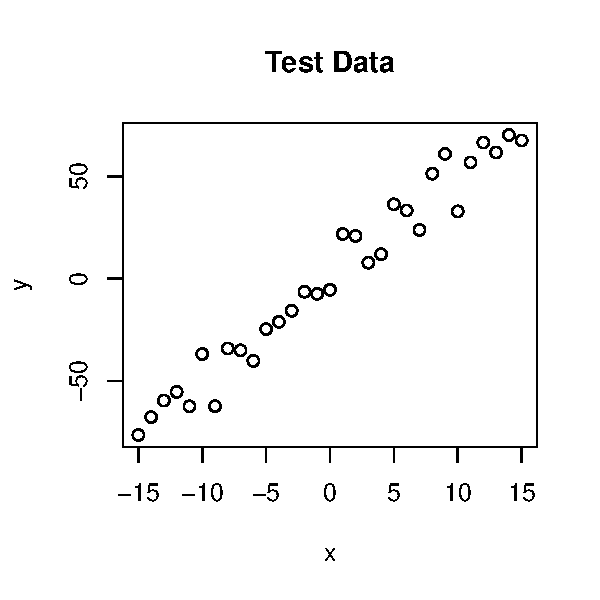
\includegraphics[width=\maxwidth]{figure/setup_parameters-1} 

}



\end{knitrout}
\caption{Plot of y against x}\label{Data}
\end{figure}

\noindent The estimation method used with the Metropolis-Hastings algorithm later is actually an application of the Maximum Likelihood (ML) method. It can be shown that the OLs estimators and the MLE estimators in the case of a Linear Model are the same. The ML method gives a value to the estimators by maximizing the likelihood function, or for easier computation, the log likelihood function. As an example, we will show this as a function of the parameter $a$, where we let the other variables be known. This function can be seen in Figure~\ref{loglik}. Note that the maximum is found for $a \approx 5$.

\begin{figure}[H]
\begin{knitrout}
\definecolor{shadecolor}{rgb}{0.969, 0.969, 0.969}\color{fgcolor}

{\centering 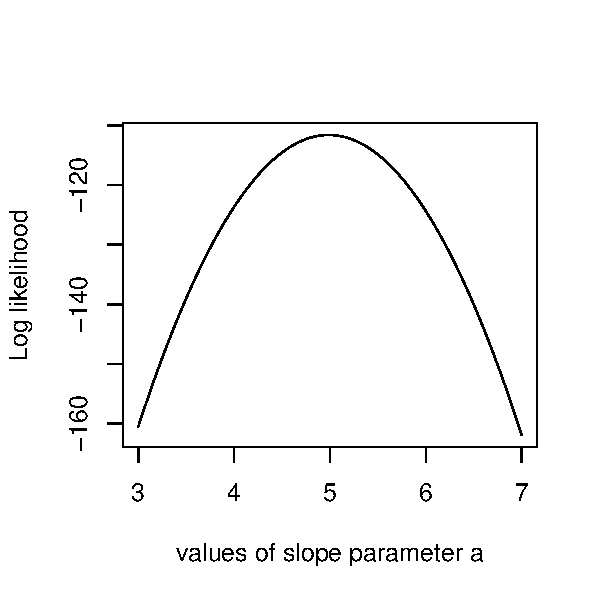
\includegraphics[width=\maxwidth]{figure/log_likelihood-1} 

}



\end{knitrout}
\caption{Log likelihood as a function of $a$}\label{loglik}
\end{figure}

\noindent Finally, the use of the actual Metropolis-Hastings algorithm will be explained. The function that we want to draw from using the algorithm, is the log likelihood function of all the parameters. Since this function maximizes at the estimates that we want, we can find the estimates by taking the mean of the values in the chain that the parameters take, as they will be spread mostly around the maximum. The example uses a Bayesian approach, so the log likelihood function is actually composed of two seperate log likelihoods, the one for the data and the one for the parameters. Also, a parameter called $burnIn$ is introduced, which is the number of values that are erased from the beginning of the chain, so that the estimates are less influenced by the arbitrary starting values. The prior distributions for the parameters and the value of $burnIn$ are shown below.

\begin{itemize}
  \item $a \sim \text{Uniform}(0,10)$
  \item $b \sim \mathcal{N}(0,5)$
  \item $\sigma \sim \text{Uniform}(0,30)$
  \item $burnIn = 5000$
\end{itemize}

\newpage
\section{Results}\label{Res}

In this section we will finally look at the some results of the algorithm. Before we compare the accuracy of the algorithm using a different number of iterations, we will first look at just one simulation. 

\subsection{One simulation}

For this particular simulation, we choose to iterate $10000$ times. In Figure~\ref{res} the results for all the parameters are shown. These results include a histogram of the amount of times that the parameters took a certain value in the chain, representing the posterior distributions. The results also include the values of the parameters in the order that they appear in the chain.

\begin{figure}[H]
\begin{knitrout}
\definecolor{shadecolor}{rgb}{0.969, 0.969, 0.969}\color{fgcolor}

{\centering 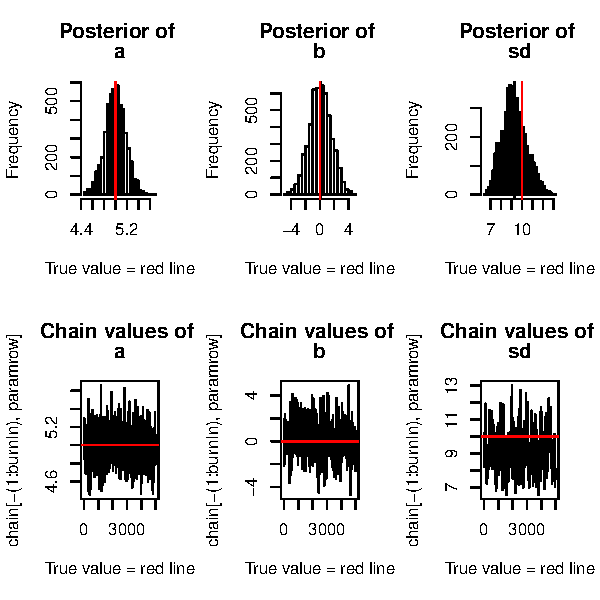
\includegraphics[width=\maxwidth]{figure/onesim-1} 

}



\end{knitrout}
\caption{Plots showing the posterior distributions and the chain values for the parameters}\label{res}
\end{figure}

\noindent The red line in all the plots show the true value of the parameters as given in Section~\ref{Set}. The estimates do seem to be slightly off from the true values, but it is actually more fair to compare the plots against the OLS estimators instead. These values fit the simulated data set more than the actual parameters, therefore it makes more sense for the estimators found using the algorithm to be closer to the OLS estimators. These can easily be computed by using the \texttt{summary(lm(\dots))} command in R.

\newpage
\begin{knitrout}
\definecolor{shadecolor}{rgb}{0.969, 0.969, 0.969}\color{fgcolor}\begin{kframe}
\begin{verbatim}
## 
## Call:
## lm(formula = y ~ x)
## 
## Residuals:
##      Min       1Q   Median       3Q      Max 
## -17.8730  -6.7328  -0.1495   5.1152  16.4052 
## 
## Coefficients:
##             Estimate Std. Error t value Pr(>|t|)    
## (Intercept)   0.4492     1.6125   0.279    0.783    
## x             4.9856     0.1803  27.653   <2e-16 ***
## ---
## Signif. codes:  0 '***' 0.001 '**' 0.01 '*' 0.05 '.' 0.1 ' ' 1
## 
## Residual standard error: 8.978 on 29 degrees of freedom
## Multiple R-squared:  0.9635,	Adjusted R-squared:  0.9622 
## F-statistic: 764.7 on 1 and 29 DF,  p-value: < 2.2e-16
\end{verbatim}
\end{kframe}
\end{knitrout}

\noindent Note that the OLS estimators are given by

\begin{itemize}
  \item $a = 4.985566$
  \item $b = 0.4491542$
  \item $\sigma = 8.9782866$
\end{itemize}

\noindent Comparing these values to the plots in Figure~\ref{res} instead, show that the estimates are actually very similar. The plot also gives a nice visualization of the standard deviations of the estimates.

\subsection{Comparing multiple simulations}

Finally we will analyze the results for a different amount of iterations for the algorithm. For this part we will only look at the estimates for the slope parameter $a$. We will look at the estimate itself, as well as its standard deviation. This will be done $10$ times for each different number of iterations, and these numbers will be $1000$, $10000$ and $100000$ iterations. 

\begin{knitrout}
\definecolor{shadecolor}{rgb}{0.969, 0.969, 0.969}\color{fgcolor}\begin{kframe}
\begin{verbatim}
## [1] "10 estimates with 1000 iterations, followed by their standard deviations"
##  [1] 4.979580 4.946759 4.975452 4.949287 5.014587 4.854780 5.025671
##  [8] 4.943863 4.951414 4.951131
##  [1] 0.1844883 0.2007029 0.2489302 0.2246267 0.1980038 0.4889043 0.1656550
##  [8] 0.1830882 0.1627742 0.2882509
\end{verbatim}
\end{kframe}
\end{knitrout}
\begin{knitrout}
\definecolor{shadecolor}{rgb}{0.969, 0.969, 0.969}\color{fgcolor}\begin{kframe}
\begin{verbatim}
## [1] "10 estimates with 10000 iterations, followed by their standard deviations"
##  [1] 4.971785 4.994001 4.990290 4.984964 4.995414 4.984716 4.987440
##  [8] 4.985517 4.985034 4.993290
##  [1] 0.2165596 0.1935525 0.2000632 0.1925966 0.1827531 0.1937681 0.2100736
##  [8] 0.1958315 0.1969475 0.2050317
\end{verbatim}
\end{kframe}
\end{knitrout}
\begin{knitrout}
\definecolor{shadecolor}{rgb}{0.969, 0.969, 0.969}\color{fgcolor}\begin{kframe}
\begin{verbatim}
## [1] "10 estimates with 100000 iterations, followed by their standard deviations"
##  [1] 4.982564 4.985454 4.977678 4.987236 4.987286 4.988064 4.986521
##  [8] 4.985172 4.986056 4.981402
##  [1] 0.1882663 0.1883190 0.1898142 0.1936325 0.1876476 0.1891106 0.1903238
##  [8] 0.1907854 0.1949303 0.1868329
\end{verbatim}
\end{kframe}
\end{knitrout}

\noindent Again we will compare these values with the OLS estimator for $a$, 4.985566, instead of the true value of $a$, $5$. Note that there is a significant difference in the accuracy of the algorithm between $1000$ iterations and the other two numbers. Also, while the estimates get better for a higher amount of iterations, and the standard deviations do get smaller, they usually still are a bit larger than the standard error of the OLs parameter of $a$, 0.1802883. This shows that an even higher amount of iterations is needed to lower the standard deviation some more. This ends the discussion of the results and with that also this report.

\end{document}
